\documentclass[11pt]{ctexart}
\usepackage[top=2cm, bottom=2cm, left=2cm, right=2cm]{geometry}
\usepackage{algorithm}
\usepackage{algorithmicx}
\usepackage{algpseudocode}
\usepackage{amsmath}
\usepackage{graphicx}
\usepackage{listings}
\usepackage{xcolor}
\usepackage{float}
\usepackage{amsmath}
\usepackage{amssymb}
\floatname{algorithm}{算法}
\renewcommand{\algorithmicrequire}{\textbf{输入:}}
\renewcommand{\algorithmicensure}{\textbf{输出:}}
\lstset{numbers=left, %设置行号位置
        numberstyle=\tiny, %设置行号大小
        keywordstyle=\color{blue}, %设置关键字颜色
        commentstyle=\color[cmyk]{1,0,1,0}, %设置注释颜色
        frame=single, %设置边框格式
        escapeinside=``, %逃逸字符(1左面的键),用于显示中文
        breaklines, %自动折行
        extendedchars=false, %解决代码跨页时,章节标题,页眉等汉字不显示的问题
        xleftmargin=2em,xrightmargin=2em, aboveskip=1em, %设置边距
        tabsize=4, %设置tab空格数
        showspaces=false %不显示空格
}
\title{\huge\bf
矩阵连乘 - 实验报告}
\author{毛圆鑫 - 201721012271}
\date{Oct 25, 2019}

\begin{document}  
\maketitle
\section*{说明}
\noindent  由于代码比较长,所以本文中的代码均以片段的形式给出,完整代码请见所附的两个.cpp文件,\\或https://github.com/punk-boy/algorithm/下的 matrixchain1.cpp和 matrixchain2.cpp\\
\noindent  还有就是本文档是使用latex语言编写的,其源文件也可见于附件或Github。


\section{伪代码}
\begin{algorithm}[H]
\caption{矩阵连乘问题 - 动态规划解法 - 伪代码}
\begin{algorithmic}[1]
\Require $P[]$矩阵维数数组,$n$矩阵的个数
\Ensure $m[1][n]$n个矩阵相乘所需的的最小数乘乘法,$s[][]$对应的数乘顺序
\Function {MatrixChain}{$p[], n$}
\For{$i=1 \to n$}
\State{$m[i][i] \gets 0$}
\EndFor
\For{$r=2 \to n$}
\For{$i=1 \to (n-r-1)$}
\State{$j\gets i+r-1$}
\State{$k\gets i$}
\State{$m[i][j]\gets m[i+1][j]+p[i-1]\times p[k] \times p[j]$}
\State{$s[i][j]\gets i$}
\For{$k=i+1 \to j$}
\State{$m[i][j]\gets \min\{m[i][j],m[i][k-1]+m[k][j]+p[i-1]\times p[k] \times p[j]\}$}
\State{$s[i][j]\gets \min\{k | m[i][j],m[i][k-1]+m[k][j]+p[i-1]\times p[k] \times p[j]\}$}
\EndFor
\EndFor
\EndFor
\State{$return m[1][n], S$}
\EndFunction
\end{algorithmic}
\end{algorithm}


\section{基本测试}
\noindent  这次的代码实现比较简单比较简单,我就随便的粘一部分用于说明,具体详细代码请看源文件。
\subsection{MatrixChain函数}
\begin{lstlisting}[language=C++]
int matrix_chain(int * p, int n)
{
	int ** m = (int **)malloc(sizeof(int *) * n);
	s = (int **)malloc(sizeof(int *) * n);
	for(int i=0;i<n;i++)
	{
		m[i] = (int *)malloc(sizeof(int) * n);
		s[i] = (int *)malloc(sizeof(int) * n);
	}
	for(int i=0;i<n;i++)
		m[i][i] = 0;		
	for(int r=2;r<=n;r++)
	{
		for(int i=0;i<n-r+1;i++)
		{
			int j = i+r-1;
			int k = i;
			m[i][j] = m[i+1][j] + p[i-1] * p[k] * p[j];
			s[i][j] = i;
			for(k=i+1;k<=j;k++)
			{
				if(m[i][j] > m[i][k-1] + m[k][j] + p[i-1]*p[k]*p[j])
				{
					m[i][j] = m[i][k-1] + m[k][j] + p[i-1]*p[k]*p[j];
					s[i][j] = k;
				}
			}
		}
	}
	return m[1][n-1];
}
\end{lstlisting}

\subsection{监控结果和时间的部分}
\begin{lstlisting}[language=C++]
start = clock();
int result = matrix_chain(p, plen);
end = clock();
for(int i=0;i<plen;i++) printf("%d\t",p[i]);
printf("\nresult = %d\n", result);
printf("time consumed : %.2lf seconds\n", 1.0 * (end - start) / CLOCKS_PER_SEC);
\end{lstlisting}
\subsection{运行结果}
\begin{figure}[H]
\centering
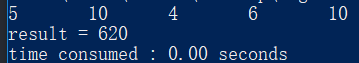
\includegraphics{3.png}
\caption{基本测试的实验结果}
\end{figure}

\section{复杂的测试}
\noindent  这个算法在$n=10000$时,我的电脑就已经无法在可接受的时间内运行出结果了,所以这次的复杂测试我取的时$n=1000$,但是对应的又出现了一个问题就是,高度的计算使得$int$无法存储下一个巨大的数字,我就使用了$long long$来存储数据,但是很遗憾的是,即使在$n=100$时,$long long$也无法存储下这么大的数据,所以,这里留个疑问怎么样可以存储的下那么大的数据(在不用字符串模拟的前提下),但是我还是把这个记录在实验报告中吧。
\subsection{数据生成部分}
\begin{lstlisting}[language=C++]
const int plen = 1000;
int p[plen];
for(int i=0;i<plen;i++)
	p[i] = rand() % range;
\end{lstlisting}

\subsection{MatrixChain函数}
\begin{lstlisting}[language=C++]
LL matrix_chain(int * p, int n)
{
	LL ** m = (LL **)malloc(sizeof(LL *) * n);
	s = (LL **)malloc(sizeof(LL *) * n);
	for(int i=0;i<n;i++)
	{
		m[i] = (LL *)malloc(sizeof(LL) * n);
		s[i] = (LL *)malloc(sizeof(LL) * n);
	}
	for(int i=0;i<n;i++)
		m[i][i] = 0;		
	for(int r=2;r<=n;r++)
	{
		for(int i=0;i<n-r+1;i++)
		{
			int j = i+r-1;
			int k = i;
			m[i][j] = m[i+1][j] + p[i-1] * p[k] * p[j];
			s[i][j] = i;
			for(k=i+1;k<=j;k++)
			{
				if(m[i][j] > m[i][k-1] + m[k][j] + p[i-1]*p[k]*p[j])
				{
					m[i][j] = m[i][k-1] + m[k][j] + p[i-1]*p[k]*p[j];
					s[i][j] = k;
				}
			}
		}
	}
	return m[1][n-1];
}
\end{lstlisting}

\subsection{监控结果和时间的部分}
\begin{lstlisting}[language=C++]
start = clock();
LL result = matrix_chain(p, plen);
end = clock();
for(int i=0;i<plen;i++) printf("%d\t",p[i]);
printf("\nresult = %ld\n", result);
printf("time consumed : %.2lf seconds\n", 1.0 * (end - start) / CLOCKS_PER_SEC);
\end{lstlisting}

\subsection{运行结果}
\begin{figure}[H]
\centering
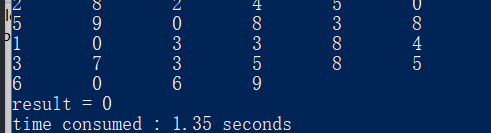
\includegraphics{4.png}
\caption{复杂的测试的实验结果}、
\end{figure}
\noindent  我们可以看到时间上的确被消耗了,但实际上由于计算机的数据存储问题没有解绝,所以我们并没有的到一个正确的答案,这里先埋个坑,留着以后填吧。


\section{感想}
这个矩阵乘法的动态规划算法跟我的那道大作业的题目十分的相似,我在大作业中提到了,对于类似问题可以采用\textbf{平行四边形优化},所以这道题目也是可以使用的,再埋个坑,以后填,先交作业:)。

\end{document}



